\section{Methodology}\label{Sec:Method}

\subsection{The Bandt-Pompe Methodology}

Let ${\mathcal X} \equiv \{x_t\}_{t=1}^{T}$ be a real valued time series of length $T$, without ties. 
As stated
by~\citeauthor{Bandt2002Permutation}~\citeyear{Bandt2002Permutation}in their seminal work:  
\begin{quote}
``If the $\{x_t\}_{t=1}^{T}$ attain infinitely many values, it is common to replace them by a symbol sequence 
$\Pi \equiv \{\pi_j\}$ with finitely many symbols, and calculate source entropy from it".
\end{quote}
Also, as stressed by these authors, 
\begin{quote}
``The corresponding symbol sequence must come 
naturally from the $\{x_t\}_{t=1}^{T}$ without former model assumptions".
\end{quote}

Let ${\mathbbm A}_{D}$ (with $D \geq 2$ and $D \in {\mathbbm Z}$) be the symmetric group of order $D!$ formed by all 
possible permutation of order $D$, and the symbol component vector 
${\bm \pi}^{(D)} = (\pi_1, \pi_2, \dots, \pi_D)$ so every element ${\bm \pi}^{(D)}$ is unique 
($\pi_j \neq \pi_k~\forall~j \neq k$). 
Consider for the time series ${\mathcal X} \equiv \{x_t\}_{t=1}^{T}$ its time delay embedding representation,
with embedding dimension $D \geq 2$ ($D \in {\mathbbm Z}$) and time delay $\tau \geq 1$ ($\tau \in {\mathbbm Z}$, also called ``embedding time''):
\begin{equation} 
\label{eq:time-delay}
{\mathbf X}^{(D,\tau)}_t ~=~( x_t,x_{t+\tau},\dots,x_{t+(D-1)\tau} ) \ ,
\end{equation} 
for $t = 1,2,\dots,N$ with $N = T-(D-1) \tau$.
Then the vector ${\mathbf X}^{(D,\tau)}_t$ can be mapped to a symbol vector ${\bm \pi}^{(D)} \in {\mathbbm A}_{D}$. 
This mapping should be defined in a way that preserves the desired relation between the elements 
$x_t  \in {\mathbf X}^{(D,\tau)}_t$, and all $t \in T$ that share this pattern (also called motif) have to mapped to the same 
${\bm \pi}^{(D)}$. 
The two most frequent ways to define the mapping ${\mathbf X}^{(D,\tau)} \mapsto {\bm \pi}^{(D)}$ are:  
\begin{enumerate}[a)]
\item ordering the ranks of the $x_t \in {\mathbf X}^{(D,\tau)}$ in chronological order 
       (\textit{Rank Permutation}) or,
\item ordering the time indexes according to the ranks of $x_t \in {\mathbf X}^{(D,\tau)}$  
       (\textit{Chronological Index Permutation});
\end{enumerate}
       see details in \citeauthor{Traversaro2018Bandt}~\ycite{Traversaro2018Bandt}.
Without loss of generality, in the following we will only use the latter.

Consider, for instance, the time series $\mathcal X = (1.8, 1.2, 3.2, 4.8, 4.2, 4.5, 2.3, 3.7, 1.2, .5)$ depicted in Fig.~\ref{Fig:IntroBP}.
Assume we are using patterns of length $D=5$ with unitary time lag $\tau=1$.
The code associated to $\mathbf X_{3}^{(5,1)}=(x_3,\dots,x_7)=(3.2, 4.8, 4.2, 4.5, 2.3)$, shown in black, is formed by the indexes in $\bm\pi^{(5)}=(1,2,3,4,5)$ which sort the elements of $\mathbf X_{3}^{(5,1)}$ in increasing order: $51342$.
With this, $\widetilde{\pi}^{(5)} = 51342$, and we increase the counting related to this motif in the histogram of all possible patterns of size $D=5$.

The dash-dot line in Fig.~\ref{Fig:IntroBP} illustrates $\mathbf X_{1}^{(5,2)}$, i.e. the sequence of length $D=5$ starting at $x_1$ with lag $\tau=2$.
In this case, $\mathbf X_{1}^{(5,2)}= (1.8, 3.2, 4.2, 2.3, 1.2)$, and the corresponding motif is $\widetilde{\pi}^{(5)}=51423$.

\begin{figure}[H]
\centering
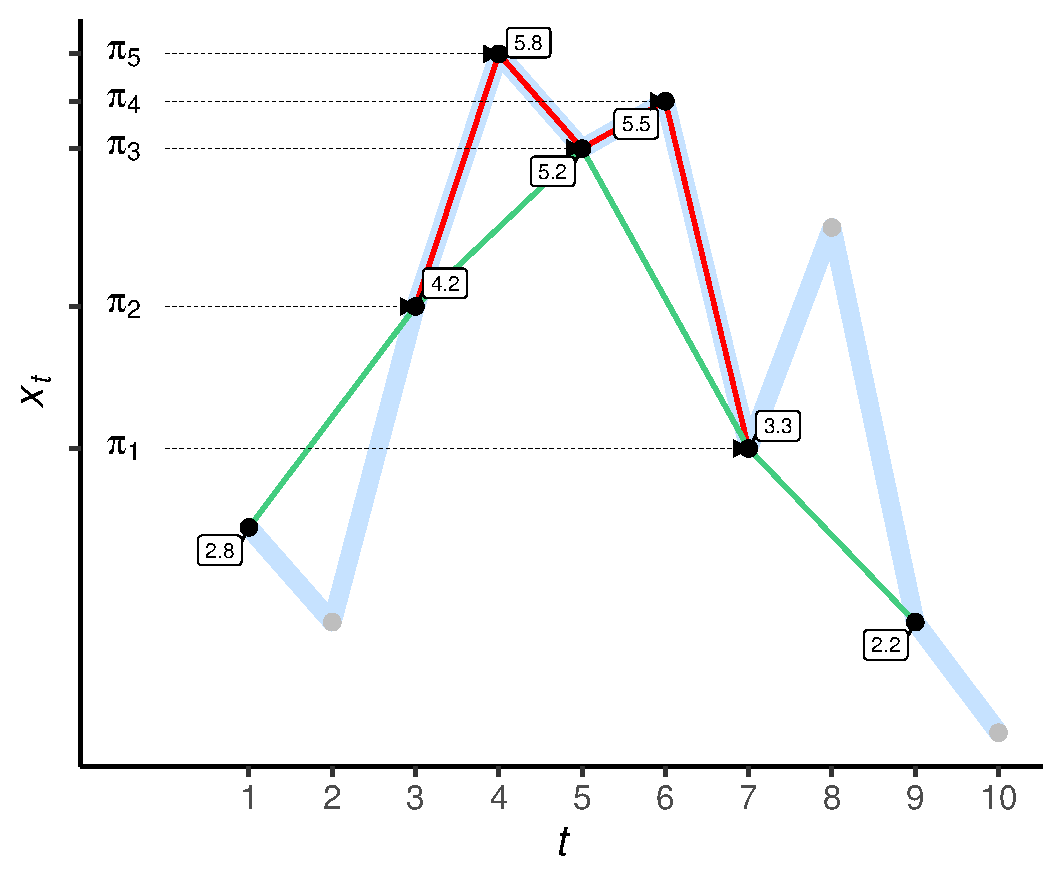
\includegraphics[width=.7\linewidth]{IntroBP}
\caption{Illustration of the Bandt and Pompe coding}
\label{Fig:IntroBP}
\end{figure}

Once all symbols have been computed, one obtains the histogram of proportions $\bm h = (h(j))_{1\leq j\leq D!}$.
This is an estimate of the (unknown, in general) probability distribution function of these patterns.
The next step into the characterization of the time series is computing descriptors from this histogram.

The first descriptor is a measure of the disorder of the system.
The most frequently used feature for this is the Normalized Shannon entropy, defined as
\begin{equation}
H(\bm h) = -\frac{1}{\log D!} \sum_{j=1}^{D!} h(j) \log h(j),
\end{equation}
with the convention that terms in the summation for which $h(j)=0$ are null.
This quantity is bounded in the unit interval, and is zero when $h(j)=1$ for some $j$ (and, thus, all other bins are zero), and one when $h(j)=1/D!$ for every $j$ (the uniform probability distribution function).

Although very expressive, the Normalized Shannon Entropy is not able to describe all possible underlying dynamics.
In particular, for intermediate values of $H$, there is a wide variety of situations worth characterizing.
To this aim, \citeauthor{LopezRuiz1995}~\citeyear{LopezRuiz1995} proposed using $Q$, the disequilibrium, a measure of how far $\bm h$ is from an equilibrium or noninformative distribution.
They employed the Euclidean distance between $\bm h$ and the uniform probability distribution function.

With this, they proposed $C=HQ$ as a measure of the Statistical Complexity of the underlying dynamics.
A time series can then be mapped into a point in the $H\times C$ plane.


\subsection{The Entropy-Complexity Plane}

We illustrate the use of the Entropy-Complexity ($H\times C$) with the following time series:
\begin{itemize}
\item Colored $k$-noise: white ($k=0$), $k=-1/2$, pink ($k=1$), $k=3/2$, red ($k=2$), $=5/2$, and $k=3$;
\item Chaotic logistic series $x_t = r x_{t-1} (1 - x_{t-1})$, with $r=3.6$ and $4$;
\item Deterministic series: monotonic increasing ($\log(x_t+0.1)$, $x_t=\{1,2,\dots,10^4$) and periodic ($\sin(2x_t)\cos(2x_t)$, with $0\leq x_t\leq 2\pi$ over ten thousand equally spaced points).
\end{itemize}
In all cases, we used $D=6$ and $\tau=1$.
Fig.~\ref{fig:Histograms} shows nine of the histograms produced by these series using the Mersenne-Twister pseudorandom number generator;
we omitted those corresponding to the deterministic series, as they produce one and two nonzero bins.

\begin{figure}[H]
\centering
	\subfloat[Logistic map $r=3.6$]{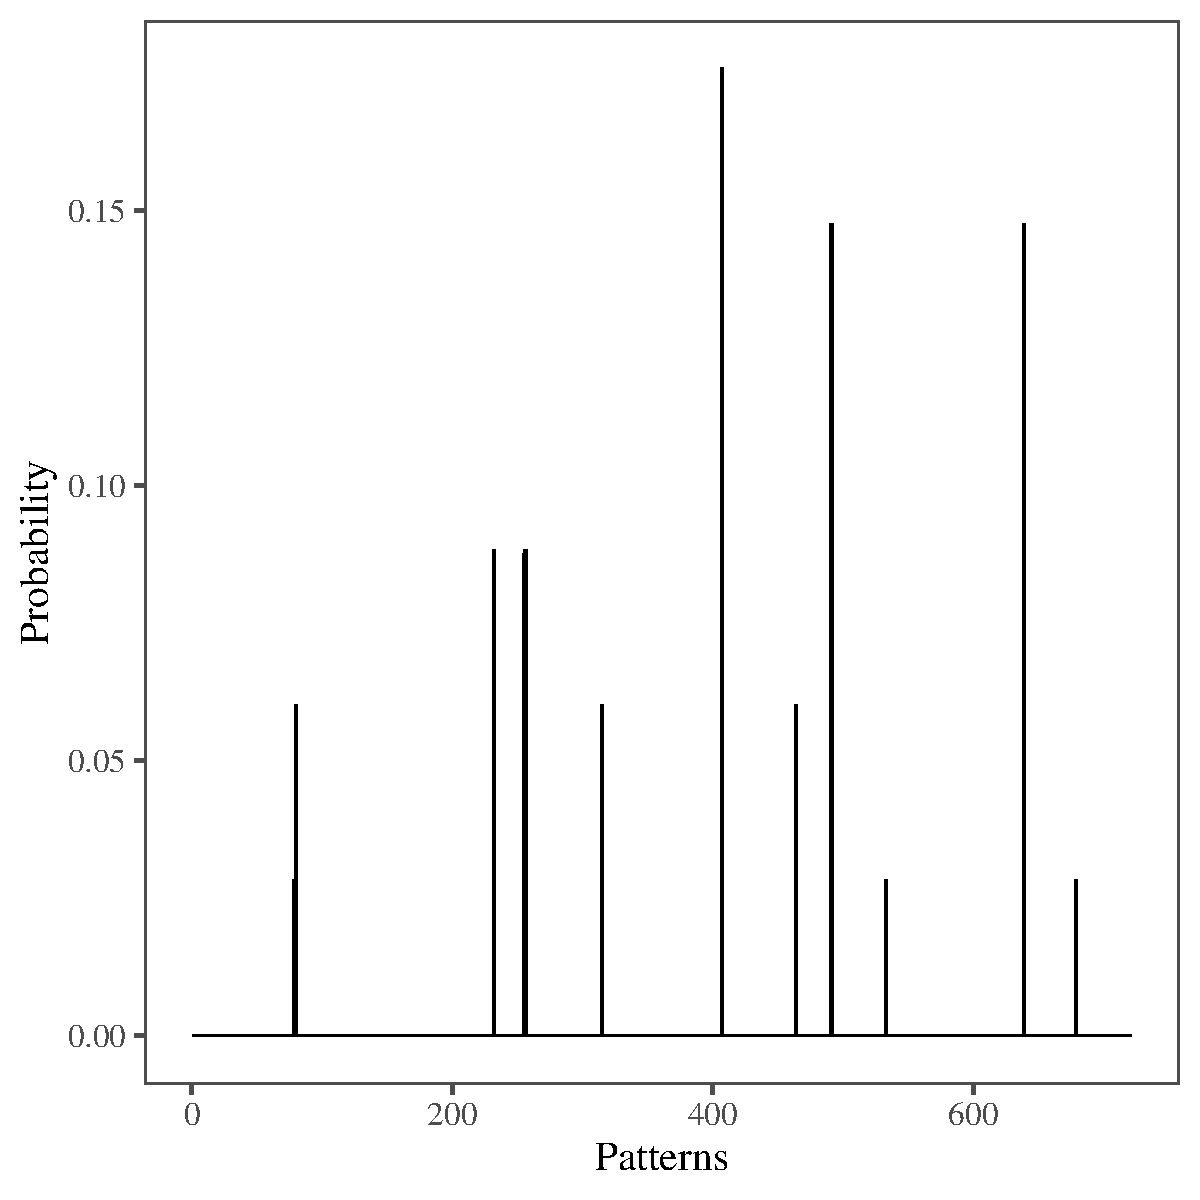
\includegraphics[width=.3\linewidth]{h36}}\quad
	\subfloat[Logistic map $r=4$]{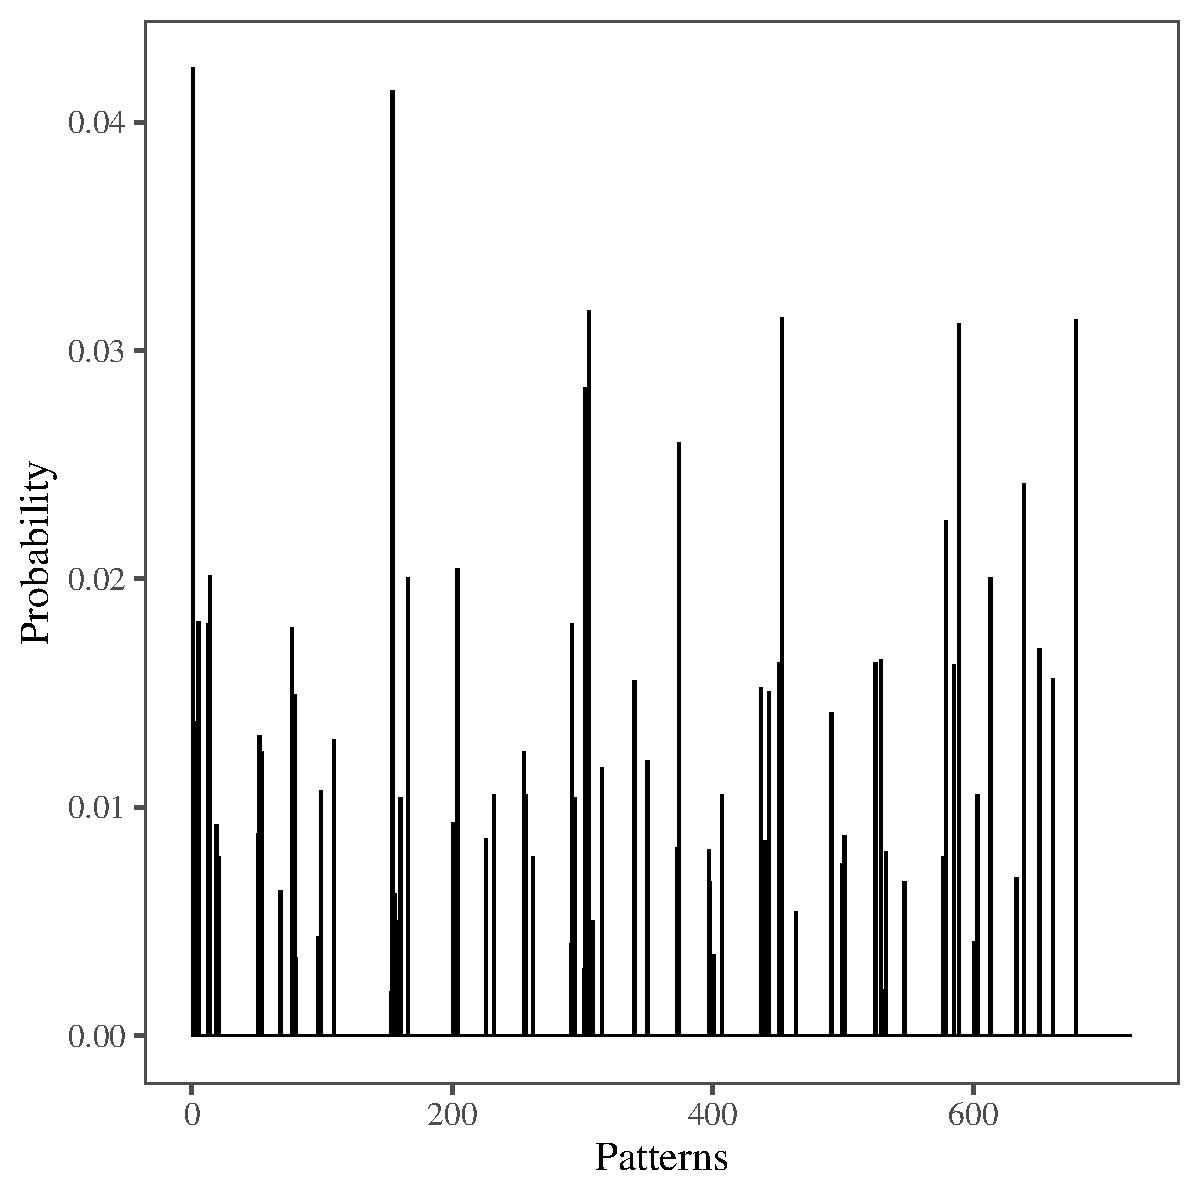
\includegraphics[width=.3\linewidth]{h4}}\quad
	\subfloat[$f^{-3}$ noise]{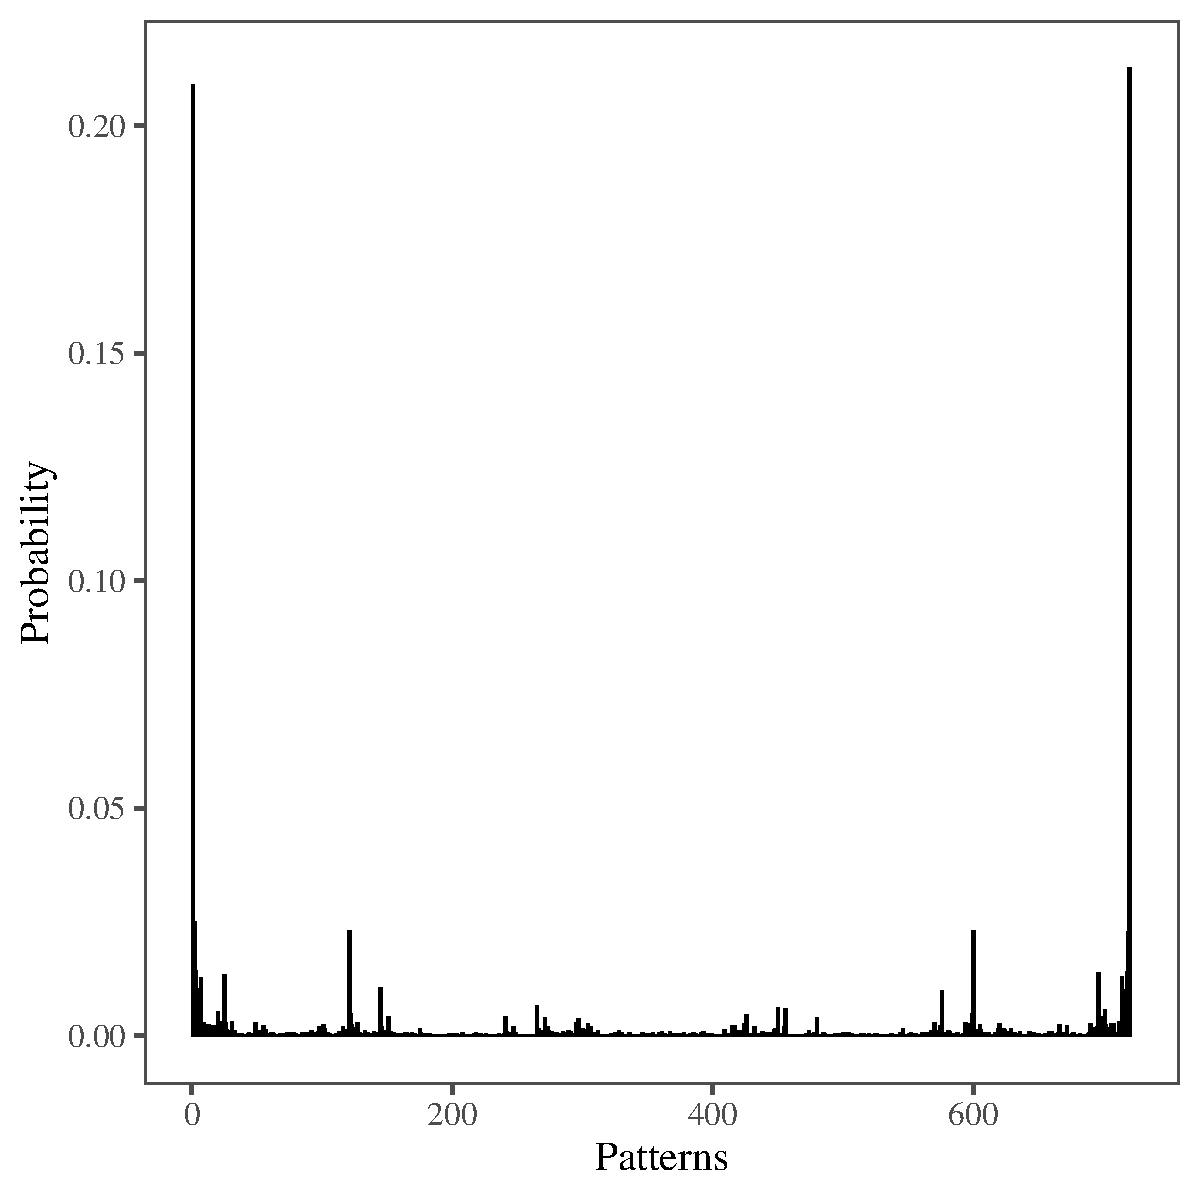
\includegraphics[width=.3\linewidth]{h3}}\quad
	\subfloat[$f^{-5/2}$ noise]{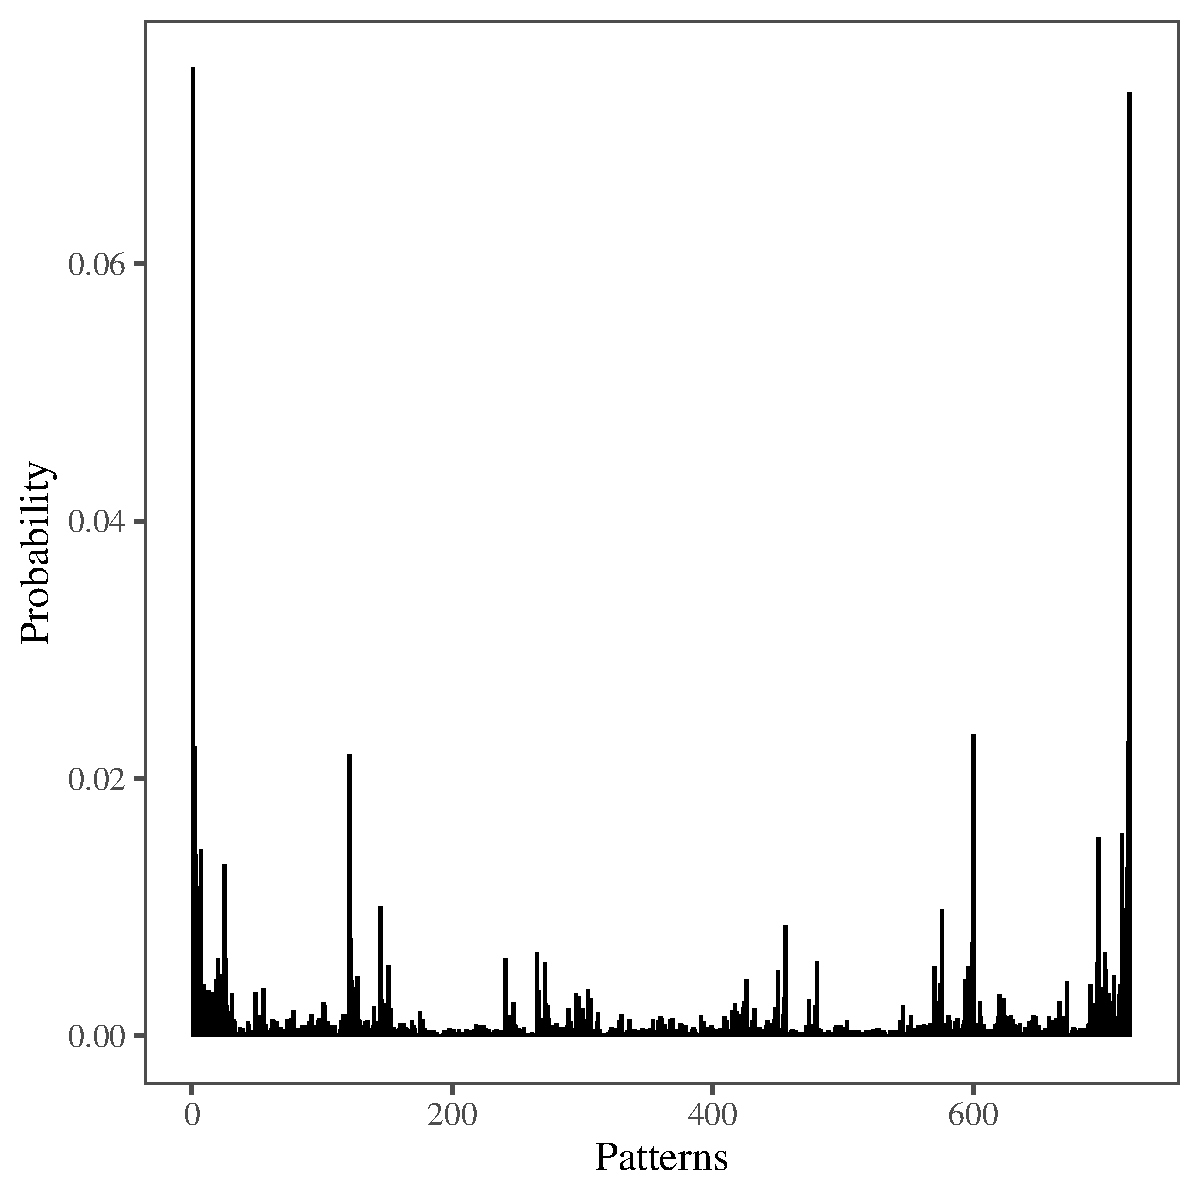
\includegraphics[width=.3\linewidth]{h25}}\quad
	\subfloat[$f^{-2}$ noise]{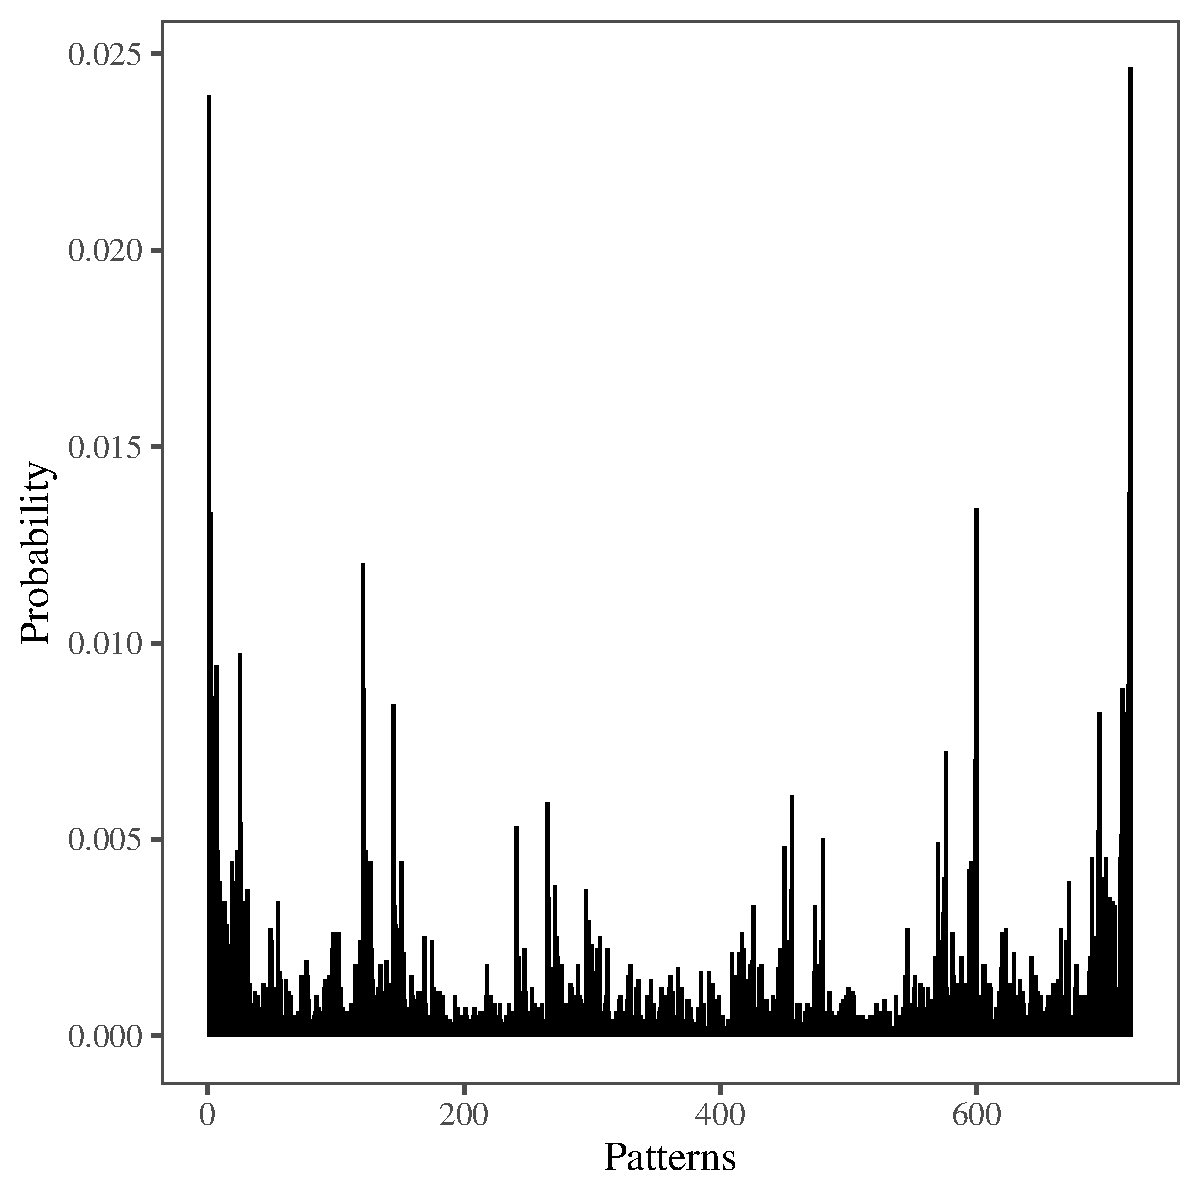
\includegraphics[width=.3\linewidth]{h2}}\quad
	\subfloat[$f^{-1.5}$ noise]{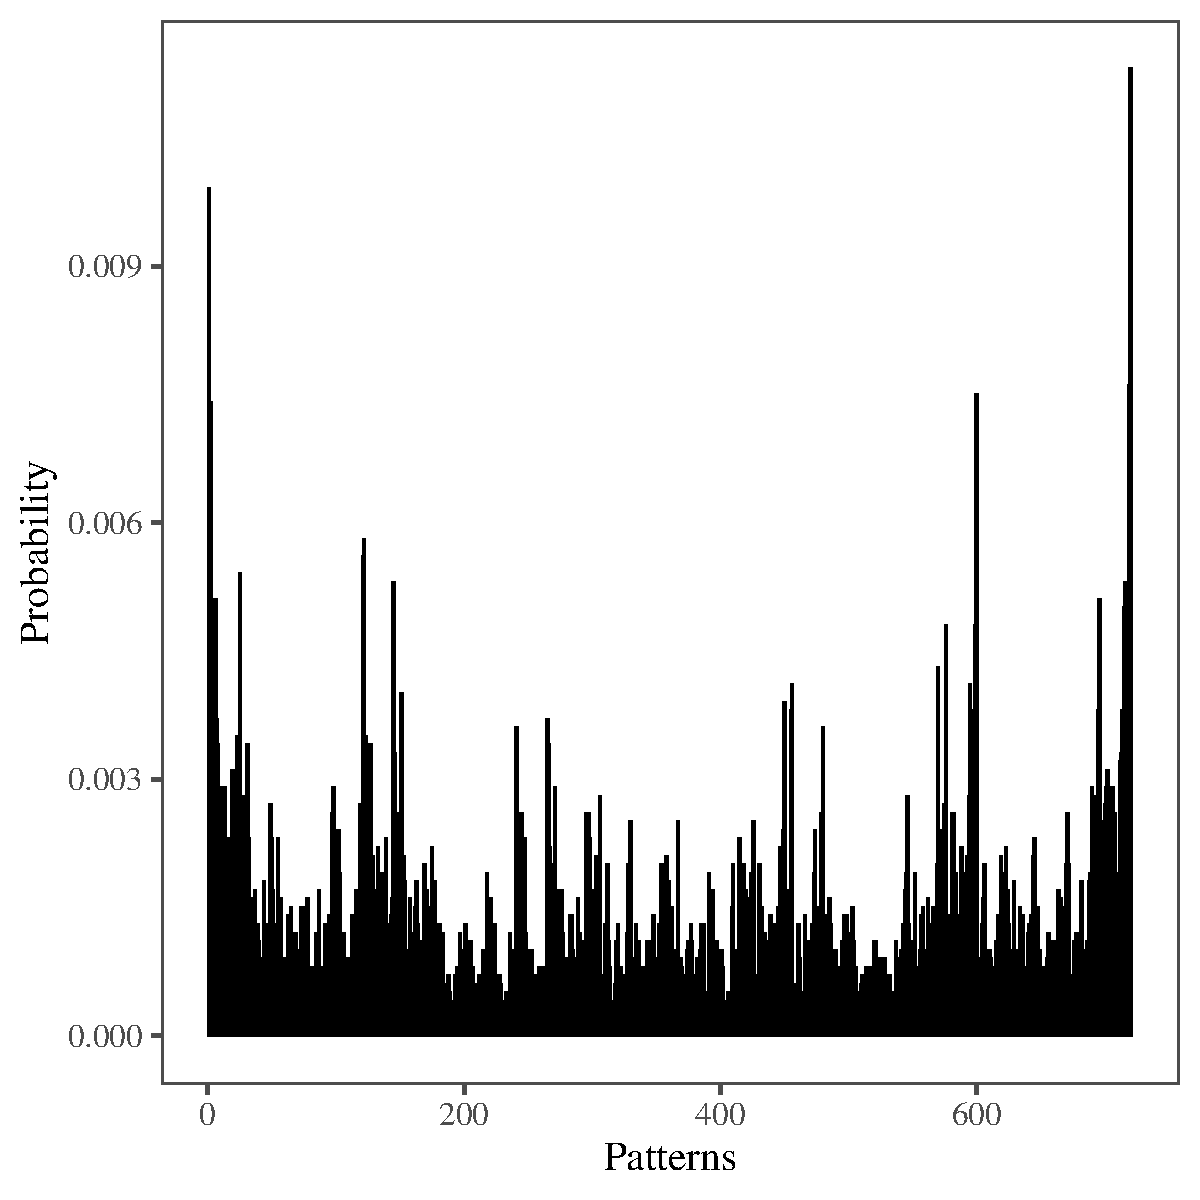
\includegraphics[width=.3\linewidth]{h15}}\quad
	\subfloat[$f^{-1}$ noise]{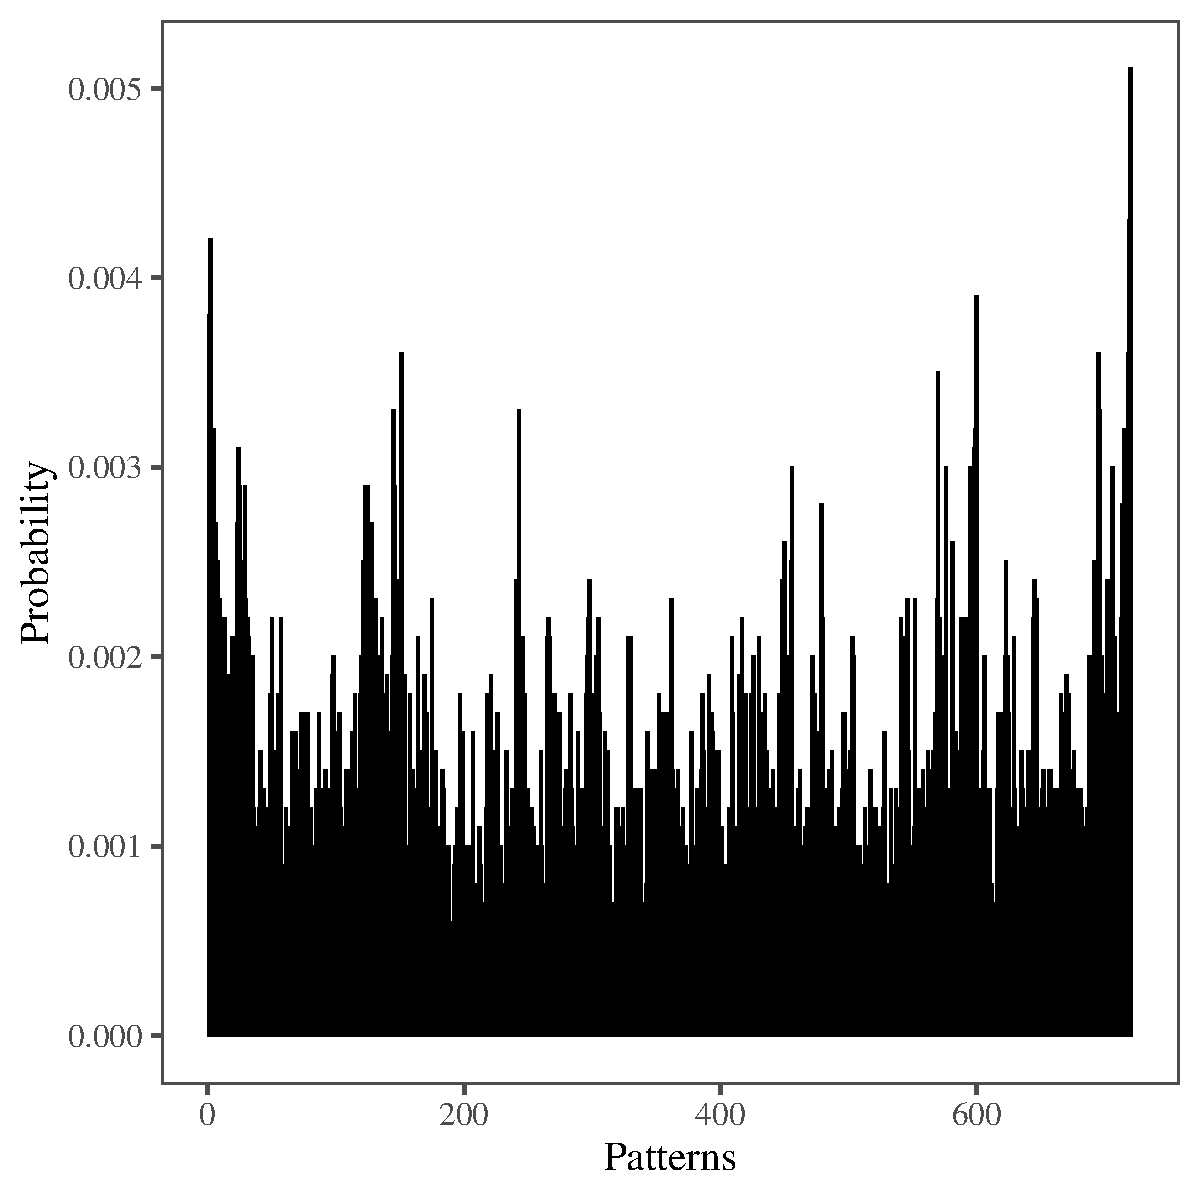
\includegraphics[width=.3\linewidth]{h1}}\quad
	\subfloat[$f^{-1/2}$ noise]{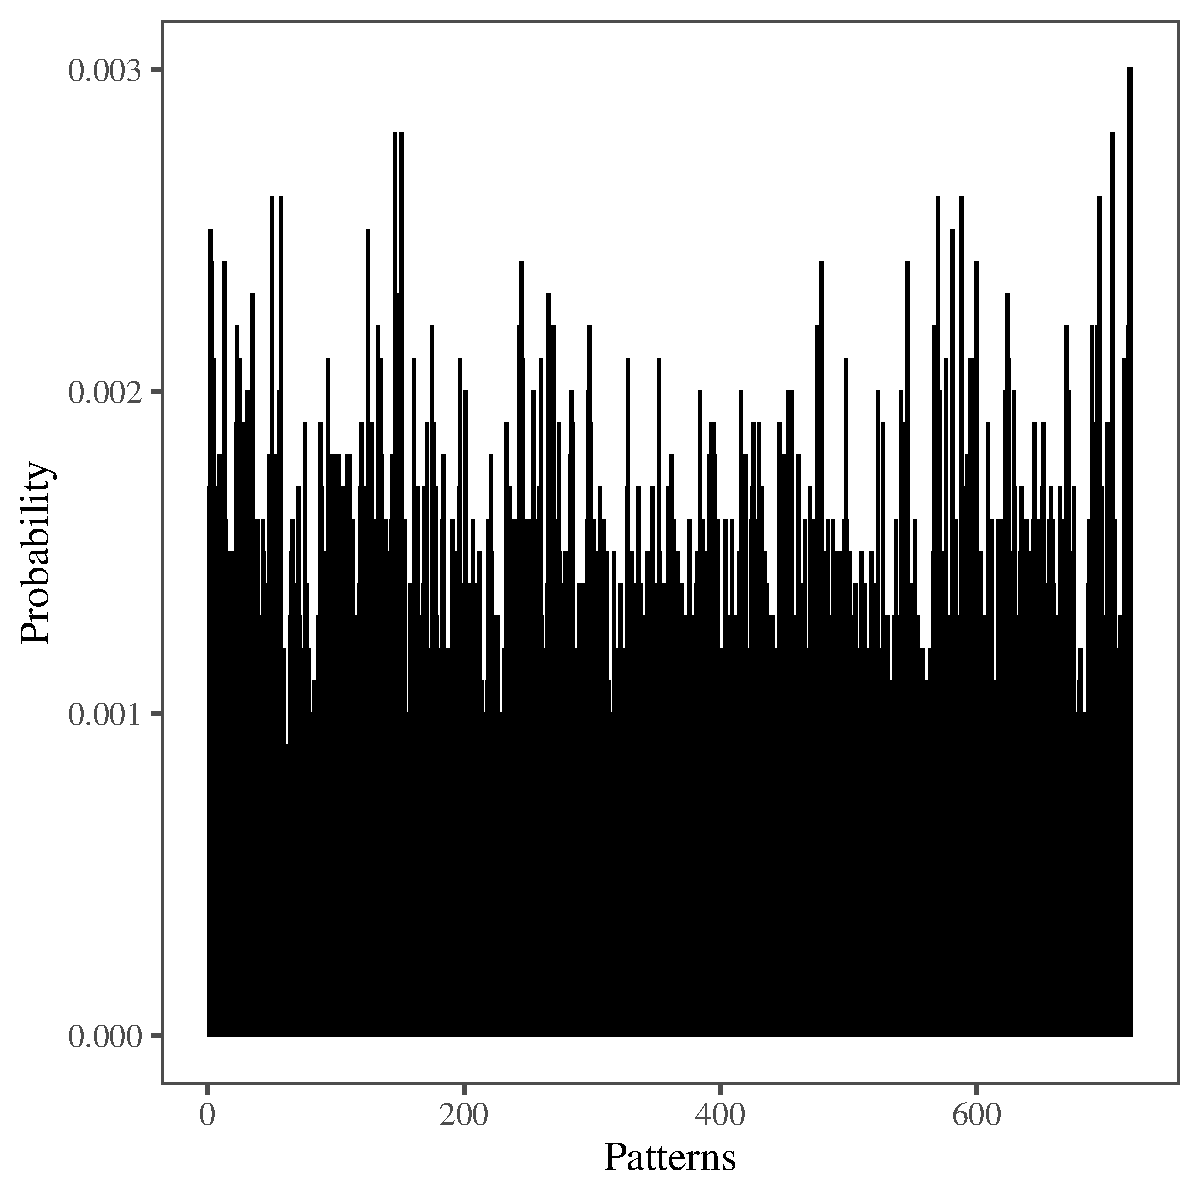
\includegraphics[width=.3\linewidth]{h05}}\quad
	\subfloat[White noise]{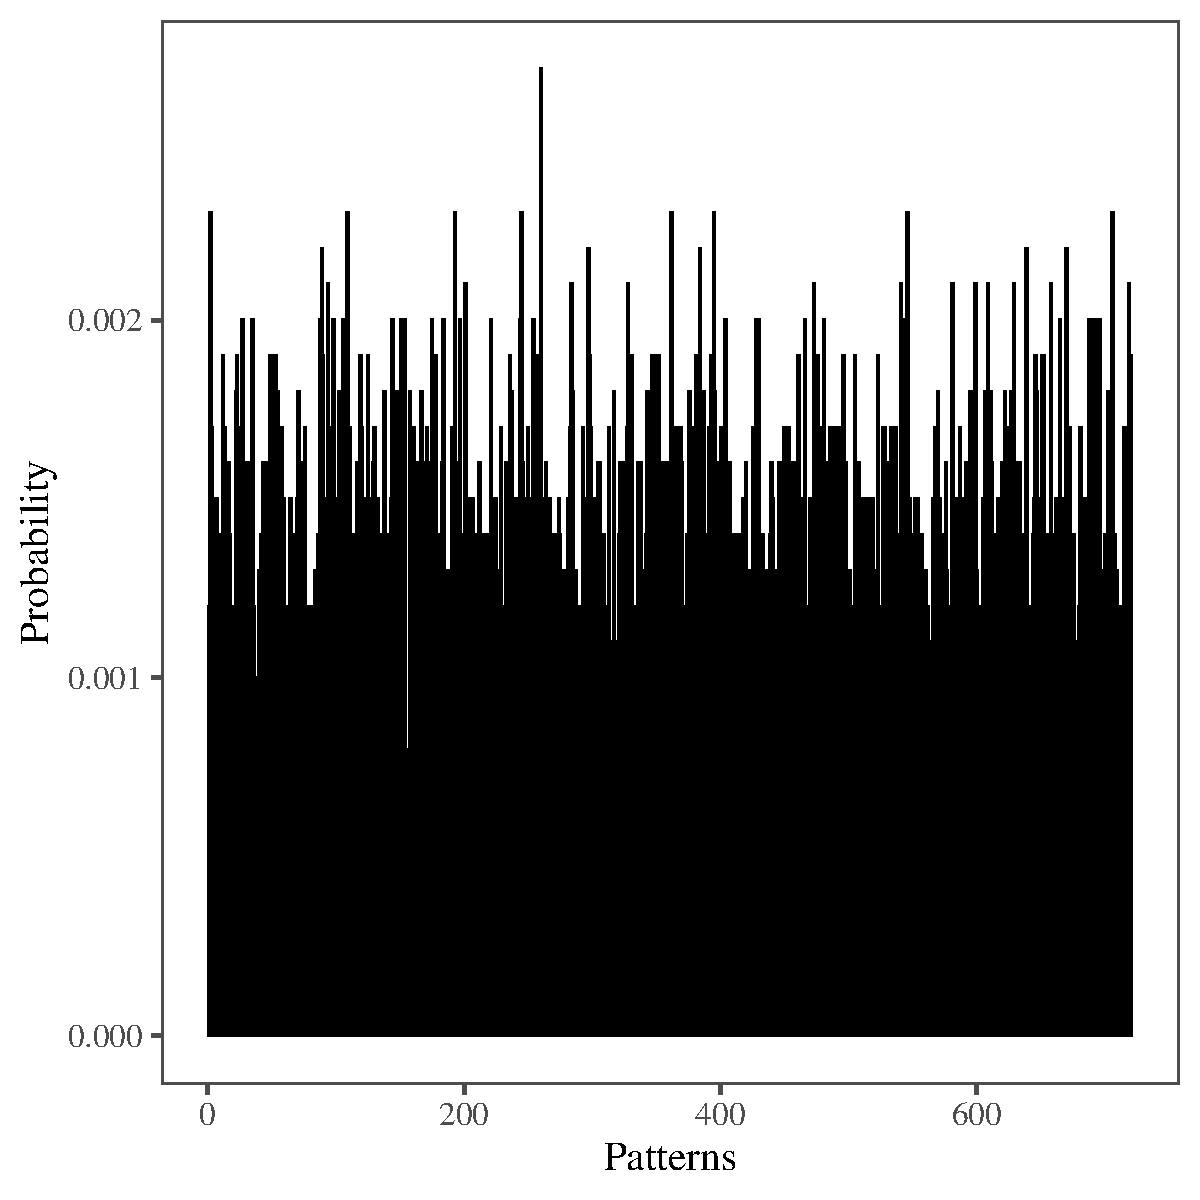
\includegraphics[width=.3\linewidth]{h0}}
	\caption{Patterns histograms of selected time series, with $D=6$ and $\tau=1$\label{fig:Histograms}}
\end{figure}


Fig.~\ref{fig:AllSystems} shows the $H\times C$ plane with the bounds for $D=6$, the time series and the points they were mapped onto.
The points due to $f^{-k}$ noises appear joined by dotted segments.
It is noticeable that deterministic patterns have more complexity than random ones.
Also, points related to $f^{-k}$ noises tend to clutter for $k<1$.

\begin{figure}[H]
\centering
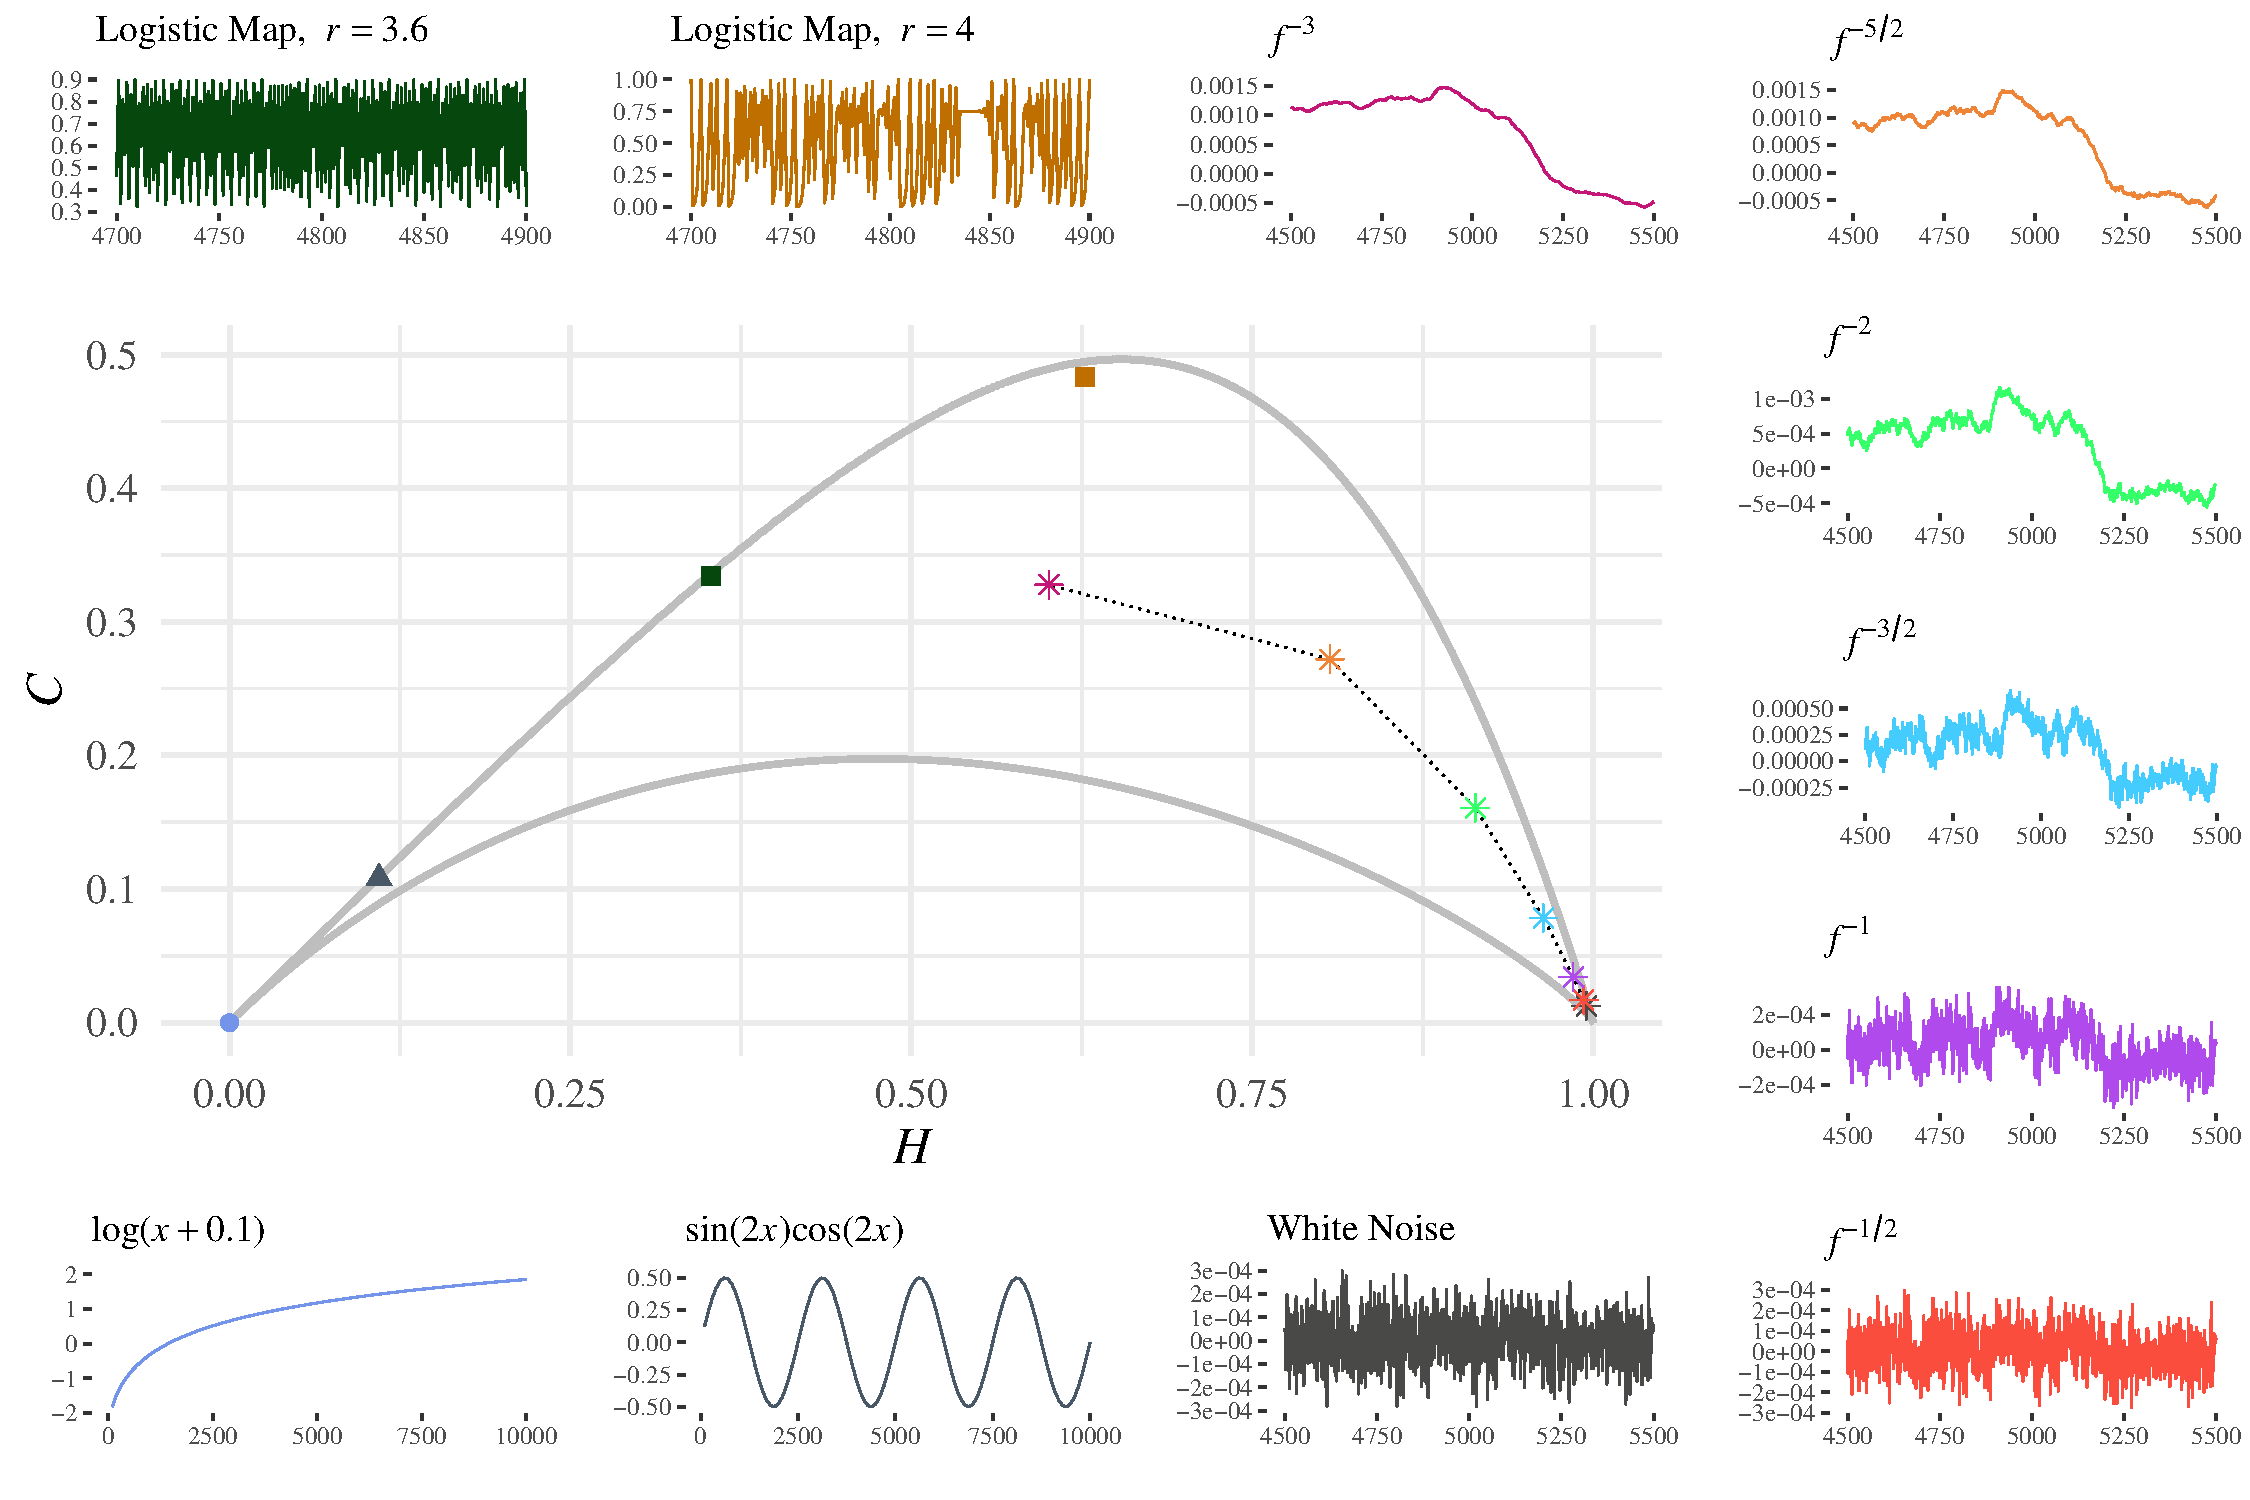
\includegraphics[width=\linewidth]{AllSystems}
\caption{Eleven systems and their points in the $H\times C$ plane}\label{fig:AllSystems}
\end{figure}

Fig.~\ref{fig:RightMostCorner} shows the rightmost lower corner of the $H\times C$ plane, emphasizing the location of the white ($k=0$), $k=-1/2$, and pink ($k=1$) noises.

\begin{figure}[H]
\centering
\includegraphics[width=\linewidth]{RightMostCorner}
\caption{White Noise, $f^{-1/2}$ and $f^{-1}$ noise points}\label{fig:RightMostCorner}
\end{figure}

The focus of our study is the empirical distribution of points produced by White and selected $f^{-k}$ noises, with this, providing confidence regions in the $H\times C$ plane.
In particular, we are interested in assessing pure randomness with this technique.

\subsection{The $H\times C$ plane in the literature}

Table~\ref{Tab:Literature} presents references in which the authors analyze time series of size $N$ and embedding dimension $D$.
The authors also attest whether the time series is white noise or not, according to its $(h,c)$ feature.

The following widely used non-chaotic algorithmic generators are analyzed:
\begin{itemize}
    \item[$-$] RNG available in Intel fortran compiler (FOR)
    \item[$-$] RNG available in Borland C++ compiler (CCC)
    \item[$-$] Matlab RAND function (MAT)
    \item[$-$] Mother RNG, available in Marsaglia website~\cite{marsaglia1994yet} (MOT)
    \item[$-$] Multiple with carry RNG (MWC)~\cite{marsaglia1994yet}
    \item[$-$] Combo RNG (COM)~\cite{marsaglia1994yet}
    \item[$-$] Lehmer RNG (LEH)~\cite{payne1969coding}
    \item[$-$] Fractional Gaussian noise with $\alpha = 0$ (fGn)
    \item[$-$] Fractional Brownian motion with $\alpha = 1.2$ (fBm)
    \item[$-$] $f^{-k}$ noise with $k = 0$
    \item[$-$] Linear Congruential Generator (LCG)~\cite{knuth1997sorting}
\end{itemize}

\begin{table}[H]
    \caption{References which attest whether a time series of size $N$ is white noise according to its $(h,c)$ feature, and the empirical $p$-value of such hypothesis according to our results}
    \label{Tab:Literature}
    \centering
    \begin{tabular}{llcccccc}
    \toprule
Reference & PRNG & $N$ & $D$ & $H$ & $C$ & Is white noise? & $p$-value\\ 
\midrule
\citeauthor{larrondo2002statistical} (\citeyear{larrondo2002statistical}) &  MOT & NA & 6 & $\cong 0.9969$ & $\cong 0$ & no & NA\\
 &  FOR & NA & 6 & $\cong 0.997$ & $\cong 0$ & no & NA\\
 &  CCC & NA & 6 & $\cong 0.997$ & $\cong 0$ & no & NA\\
 &  MAT & NA & 6 & $\cong 0.997$ & $\cong 0$ & no & NA\\
\cmidrule(lr){1-8}
\citeauthor{gonzalez2005statistical} (\citeyear{gonzalez2005statistical})  &  MWC & 65536 & NA & $\cong 1$ & $0.3$ & yes & NA\\
 &  MOT & 65536 & NA & $\cong 1$ & $0.3$ & yes & NA\\
 &  COM & 65536 & NA & $\cong 1$ & $0.05$ & yes & NA\\
\cmidrule(lr){1-8}
\citeauthor{Larrondo2006Random} (\citeyear{Larrondo2006Random}) &  LEH & \num[scientific-notation=true]{5 e6} & 5 & NA & $10^{-4}$ & yes & NA\\
 &  MOT & \num[scientific-notation=true]{5 e6} & 5 & NA & $10^{-4}$ & yes & NA\\
 &  MWC & \num[scientific-notation=true]{5 e6} & 5 & NA & $10^{-4}$ & yes & NA\\
\cmidrule(lr){1-8}
\citeauthor{olivares2012contrasting} (\citeyear{olivares2012contrasting}) &  fGn & \num[scientific-notation=true]{2 e15} & 6 & $\cong 0.998$ & NA & yes & NA\\
 & fBm & \num[scientific-notation=true]{2 e15} & 6 & $\cong 0.993$ & NA & yes & NA\\
 & $f^{-k}$ & \num[scientific-notation=true]{2 e15} & 6 & $\cong 0.997$ & NA & yes & NA\\
\cmidrule(lr){1-8}
\citeauthor{rosso2013characterization} (\citeyear{rosso2013characterization}) &  LCG & \num[scientific-notation=true]{1 e7} & 6 & $0.997871$ & $0.005101$ & no & NA\\
\cmidrule(lr){1-8}
\citeauthor{xiong2020complexity} (\citeyear{xiong2020complexity}) &  fGn & \num[scientific-notation=true]{2 e17} & 6 & $\cong 1$ & $\cong 0$ & yes & NA\\
 & $f^{-k}$ & \num[scientific-notation=true]{2 e17} & 6 & $\cong 1$ & $\cong 0$ & yes & NA\\
\bottomrule
    \end{tabular}
\end{table}

%The mathematical theory of markets states that fairness is characterized by white noise.

\subsection{True Random Numbers}

\textcolor{red}{Gerador - Marcelo e Heitor}

Random numbers are used in many fields, from gambling to criptography, aiming to guarantee a secure, realistic or unpredictable behavihor. 
Pseudo randomic results can be achieved by software in a deterministic way. 
But, some applications need actual random numbers (despite the somewhat elusive nature of actual randomness).
Randomness can be observed in unpredictable real world phenomena like cathodic radiation or atmospheric noise.
In this study we used two sources of real random numbers. 
The first is based on vacuum states to generate random quantum numbers described by \citeauthor{Wittmann2010generator}~(\citeyear{Wittmann2010generator}), the second one is based on atmospheric noise captured by a cheap radio receiver presented at \url{www.random.org}.

%Deixei as URLs pois não tenho o .bib ...

%The colored $k$-noise mentioned in the previous section, also known as ``correlated noise'', is such that its power spectrum has shape $f^{-k}$.
%When $k=0$, we have white noise, i.e., independent deviates.
%The larger $k$ is, the more correlated the observations are.

\subsection{Empirical Confidence Regions}

As we do not know the joint probability distribution of the pair $(h, c)$ for a sequence of random variables collectively independent and identically distributed according to a uniform law, studies involving classical bi-variate analysis, linear regression, and generalized linear models become unfeasible at this first moment.
Therefore, for the construction of our proposal, we adopted a non-parametric approach, making an empirical analysis of data obtained from physical sources and using them as our reference in the search for confidence regions.

The set of all feasible pairs in the $H \times C$ plane is found in a compact subset of $\mathbbm{R}^2$, which has limits with explicit expressions for the boundaries of this closed manifold, dependent only on the dimension of the probability space considered, that is $D!$ in the traditional Bandt-Pompe method~\cite{martin2006generalized}.
Due to such quotas, some limitations are generated, such as the absence of a representative distance metric and the difficulty of proposing confidence regions.
In view of this, it is necessary to apply an orthogonal projection in the data for a new two-dimensional coordinate system to solve these restrictions.
A classic proposal in these categories of problems is the principal component analysis (PCA) algorithm~\cite{wold1987principal}.

Let $ {\mathcal P} = \{p_n \}_{n = 1}^{N} $ be a set of $N$ observations in the $H \times C$ plane, where ${p_n} = (h_n, c_n)$ corresponds to a time series.
We apply a principal component analysis to these points and obtain $\{(u_n,v_n)\}_{n=1}^N$.
This transformation yields uncorrelated observations in the $\Omega_1\times\Omega_2$ plane.

We will find the empirical confidence regions on the $\Omega_1\times\Omega_2$ plane, and then they will be mapped back to the $H \times C$ plane.
For simplicity, and without loss of generality, assume $N$ odd; we find a parallelepiped that contains 
\SI{100}{\minusalphapercent} of the points in the $\Omega_1\times\Omega_2$ as
\begin{enumerate}
    \item Find the ranks that sort the values of the first principal component $\bm u=(u_1,u_2,\dots,u_N)$ in ascending order: $\bm r=(r_1,r_2,\dots,r_N)$, i.e., $u_{r_1}$ is the minimum value, and $u_{r_N}$ is the maximum value.
    \item Find point $(u,v)$ whose first principal component is the median: $(u_{r_{(N+1)/2}}, \cdot)$.
    \item Find the point $(u,v)$ whose first principal component is the quantile $\alpha/2$: $(u_{r_{[N\alpha/2]}}, \cdot)$.
    \item Find the point $(u,v)$ whose first principal component is the quantile $1-\alpha/2$: $(u_{r_{[N(1-\alpha/2)]}}, \cdot)$.
    \item The values $u_{r_{[N\alpha/2]}}$ and $u_{r_{[N(1-\alpha/2)]}}$ are the rightmost and leftmost bounds of the box, respectively.
    \item The top and bottom bounds of the box are the minimum and maximum values of the second principal component of the points whose first principal component is at least $u_{r_{[N\alpha/2]}}$ and at most $u_{r_{[N(1-\alpha/2)]}}$; denote these values $v_{\min}$ and $v_{\max}$, respectively.
    %\item The lower-left and upper-right corners of the box are $(u_{r_{[N\alpha/2]}}, v_{\min})$, and $(u_{r_{[N\alpha/2]}},v_{\max})$, respectively.
    \item The corners of the box are 
    $(u_{r_{[N\alpha/2]}}, v_{\min})$, 
    $(u_{r_{[N\alpha/2]}}, v_{\max})$, 
    $(u_{r_{[N(1-\alpha/2)]}}, v_{\min})$ and 
    $(u_{r_{[N(1-\alpha/2)]}},v_{\max})$.
    %\item Apply the inverse PCA transform to these corners obtaining $(h_1^{\SI{100}{\minusalphapercent}}, c_1^{\SI{100}{\minusalphapercent}})$, $(h_2^{\SI{100}{\minusalphapercent}}, c_2^{\SI{100}{\minusalphapercent}})$, $(h_1^{\SI{100}{\alphapercent}}, c_1^{\SI{100}{\alphapercent}})$ and $(h_2^{\SI{100}{\alphapercent}},c_2^{\SI{100}{\alphapercent}})$.
    \item Apply the inverse PCA transform to these corners obtaining $(h_{v_1}, c_{v_1})$, $(h_{v_2}, h_{v_2})$, $(h_{v_3}, c_{v_3})$ and $(h_{v_4},c_{v_4})$.
\end{enumerate}
These steps are also depicted in Fig.~\ref{fig:methodology}.

\begin{figure}[H]
    \centering
    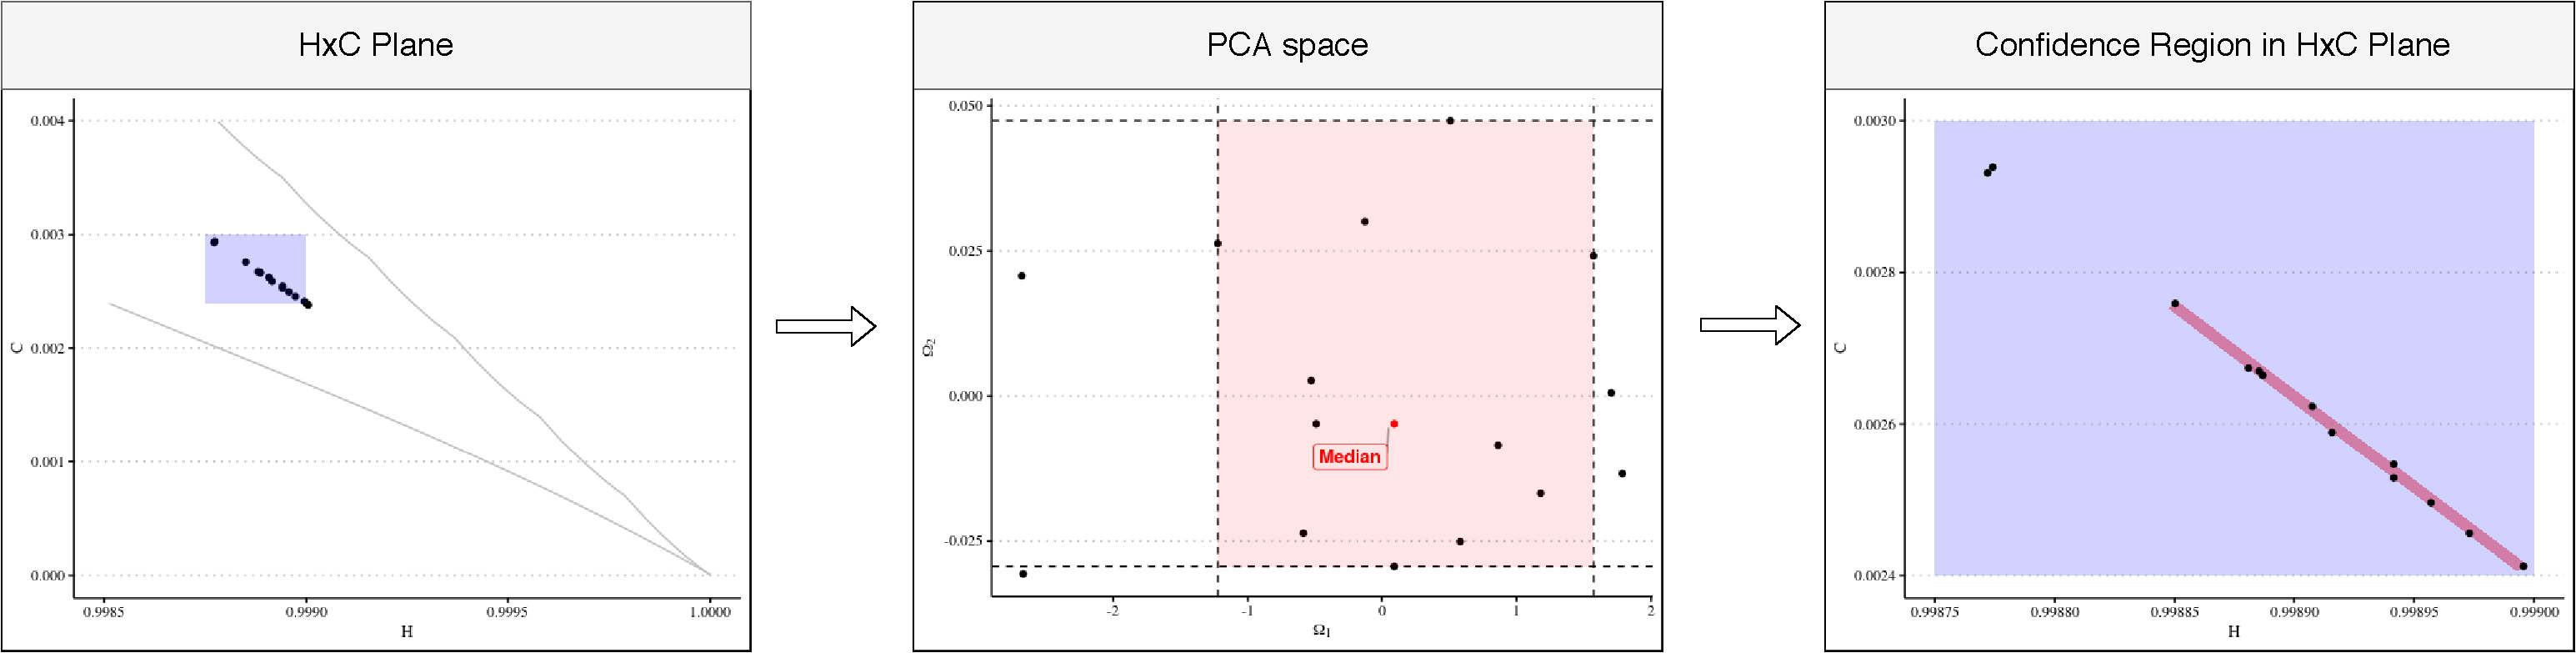
\includegraphics[width=\linewidth]{Figures/methodology.pdf}
    \caption{Outline of the methodology used for the construction of confidence regions.}
    \label{fig:methodology}
\end{figure}

\begin{sidewaystable}
    \caption{Empirical confidence regions for time series of length $T = \num[scientific-notation=true]{5 e4}$ in the $H \times C$ plane obtained by the proposed methodology}
    \label{Tab:Regions50k}
    \centering
    \begin{tabular}{cccccc}
    \toprule
Confidence Regions & $D$ & $(h_{v_1}, c_{v_1})$ & $(h_{v_2}, h_{v_2})$ & $(h_{v_3}, c_{v_3})$ & $(h_{v_4},c_{v_4})$\\ 
\midrule
\SI{90}{\percent} & 3 & $(0.9999489, \num[scientific-notation=true]{5.06e-05})$ & $(0.9999487, \num[scientific-notation=true]{5.04e-05})$ & $(0.9999998, \num[scientific-notation=true]{4e-07})$ & $(0.9999996, \num[scientific-notation=true]{2e-07})$\\
\SI{95}{\percent} & 3 & $(0.9999384, \num[scientific-notation=true]{6.11e-05})$ & $(0.9999382, \num[scientific-notation=true]{6.09e-05})$ & $(0.9999994, \num[scientific-notation=true]{9e-07})$ & $(0.9999991, \num[scientific-notation=true]{7e-07})$\\
\SI{99}{\percent} & 3 & $(0.9999079, \num[scientific-notation=true]{9.11e-05})$ & $(0.9999077, \num[scientific-notation=true]{9.09e-05})$ & $(0.9999982, \num[scientific-notation=true]{2e-06})$ & $(0.999998, \num[scientific-notation=true]{1.8e-06})$\\
\SI{99.9}{\percent} & 3 & $(0.9998625, 0.0001361)$ & $(0.9998622, 0.0001358)$ & $(0.9999973, \num[scientific-notation=true]{3e-06})$ & $(0.999997, \num[scientific-notation=true]{2.7e-06})$\\
\cmidrule(lr){1-6}
\SI{90}{\percent} & 4 & $(0.9999684, \num[scientific-notation=true]{3.98e-05})$ & $(0.9999696, \num[scientific-notation=true]{4.13e-05})$ & $(0.9998075, 0.0002508)$ & $(0.9998087, 0.0002524)$\\
\SI{95}{\percent} & 4 & $(0.9999725, \num[scientific-notation=true]{3.44e-05})$ & $(0.9999737, \num[scientific-notation=true]{3.6e-05})$ & $(0.9998506, 0.0001942)$ & $(0.9998518, 0.0001958)$\\
\SI{99}{\percent} & 4 & $(0.9999783, \num[scientific-notation=true]{2.68e-05})$ & $(0.9999795, \num[scientific-notation=true]{2.83e-05})$ & $(0.9998756, 0.0001615)$ & $(0.9998768, 0.000163)$\\
\SI{99.9}{\percent} & 4 & $(0.9999833, \num[scientific-notation=true]{2.02e-05})$ & $(0.9999845, \num[scientific-notation=true]{2.18e-05})$ & $(0.9998889, 0.000144)$ & $(0.9998901, 0.0001456)$\\
\cmidrule(lr){1-6}
\SI{90}{\percent} & 5 & $(0.9998172, 0.0003232)$ & $(0.9998194, 0.0003273)$ & $(0.9994812, 0.0009246)$ & $(0.9994834, 0.0009286)$\\
\SI{95}{\percent} & 5 & $(0.9998259, 0.0003075)$ & $(0.9998282, 0.0003116)$ & $(0.9996371, 0.0006455)$ & $(0.9996394, 0.0006495)$\\
\SI{99}{\percent} & 5 & $(0.9998428, 0.0002774)$ & $(0.999845, 0.0002814)$ & $(0.9996703, 0.0005862)$ & $(0.9996725, 0.0005901)$\\
\SI{99.9}{\percent} & 5 & $(0.9998573, 0.0002517)$ & $(0.9998593, 0.0002553)$ & $(0.9996884, 0.000554)$ & $(0.9996904, 0.0005576)$\\
\cmidrule(lr){1-6}
\SI{90}{\percent} & 6 & $(0.9990169, 0.002336)$ & $(0.9990249, 0.0023554)$ & $(0.9978983, 0.0050219)$ & $(0.9979064, 0.0050413)$\\
\SI{95}{\percent} & 6 & $(0.9990368, 0.002288)$ & $(0.9990449, 0.0023074)$ & $(0.998714, 0.0030633)$ & $(0.998722, 0.0030827)$\\
\SI{99}{\percent} & 6 & $(0.9990736, 0.0021997)$ & $(0.9990817, 0.0022191)$ & $(0.998765, 0.0029407)$ & $(0.9987731, 0.0029601)$\\
\SI{99.9}{\percent} & 6 & $(0.9991069, 0.0021197)$ & $(0.999115, 0.0021392)$ & $(0.9987884, 0.0028845)$ & $(0.9987965, 0.0029039)$\\
\bottomrule
    \end{tabular}
\end{sidewaystable}


\begin{sidewaystable}
    \caption{Empirical confidence regions for time series of length $T = \num[scientific-notation=true]{1 e3}$ in the $H \times C$ plane obtained by the proposed methodology}
    \label{Tab:Regions1000}
    \centering
    \begin{tabular}{cccccc}
    \toprule
Confidence Region & $D$ & $(h_{v_1}, c_{v_1})$ & $(h_{v_2}, h_{v_2})$ & $(h_{v_3}, c_{v_3})$ & $(h_{v_4},c_{v_4})$\\ 
\midrule
\SI{90}{\percent} & 3 & $(0.9973334, 0.0025601)$ & $(0.9974047, 0.0026304)$ & $(0.9999497, 0)$ & $(1, \num[scientific-notation=true]{5.17e-05})$\\
\SI{95}{\percent} & 3 & $(0.9967311, 0.0031343)$ & $(0.9968219, 0.0032238)$ & $(0.9999398, 0)$ & $(1, \num[scientific-notation=true]{6.12e-05})$\\
\SI{99}{\percent} & 3 & $(0.9953009, 0.0045054)$ & $(0.9954349, 0.0046375)$ & $(0.9999203, 0)$ & $(1, \num[scientific-notation=true]{8.45e-05})$\\
\SI{99.9}{\percent} & 3 & $(0.9931825, 0.0065387)$ & $(0.9933704, 0.006724)$ & $(0.9998925, 0)$ & $(1, 0.0001104)$\\
\cmidrule(lr){1-6}
\SI{90}{\percent} & 4 & $(0.994364, 0.0081246)$ & $(0.9939234, 0.0075452)$ & $(0.9994791, 0.0013982)$ & $(0.9990385, 0.0008188)$\\
\SI{95}{\percent} & 4 & $(0.9937138, 0.0089796)$ & $(0.9932534, 0.0083741)$ & $(0.9991609, 0.0018166)$ & $(0.9987005, 0.0012111)$\\
\SI{99}{\percent} & 4 & $(0.9922575, 0.0108947)$ & $(0.9917308, 0.0102022)$ & $(0.9987924, 0.0023012)$ & $(0.9982658, 0.0016087)$\\
\SI{99.9}{\percent} & 4 & $(0.9902578, 0.0135243)$ & $(0.9897312, 0.0128318)$ & $(0.9985727, 0.0025901)$ & $(0.9980461, 0.0018976)$\\
\cmidrule(lr){1-6}
\SI{90}{\percent} & 5 & $(0.9811818, 0.0321294)$ & $(0.9827429, 0.0350291)$ & $(0.9919707, 0.0120896)$ & $(0.9935319, 0.0149893)$\\
\SI{95}{\percent} & 5 & $(0.9801289, 0.0340045)$ & $(0.9817117, 0.0369446)$ & $(0.9909376, 0.0139279)$ & $(0.9925204, 0.016868)$\\
\SI{99}{\percent} & 5 & $(0.977917, 0.0377295)$ & $(0.9796031, 0.0408613)$ & $(0.9898161, 0.0156277)$ & $(0.9915021, 0.0187595)$\\
\SI{99.9}{\percent} & 5 & $(0.9753326, 0.0425299)$ & $(0.9770187, 0.0456617)$ & $(0.9892599, 0.0166608)$ & $(0.9909459, 0.0197926)$\\
\cmidrule(lr){1-6}
\SI{90}{\percent} & 6 & $(0.9121895, 0.2201993)$ & $(0.9146048, 0.2260776)$ & $(0.9443868, 0.1418373)$ & $(0.9468021, 0.1477156)$\\
\SI{95}{\percent} & 6 & $(0.9105951, 0.2239294)$ & $(0.9130413, 0.2298829)$ & $(0.9419202, 0.1476904)$ & $(0.9443663, 0.1536439)$\\
\SI{99}{\percent} & 6 & $(0.9105951, 0.2239294)$ & $(0.9130413, 0.2298829)$ & $(0.9396577, 0.1531967)$ & $(0.9421039, 0.1591502)$\\
\SI{99.9}{\percent} & 6 & $(0.9077672, 0.2305874)$ & $(0.9102595, 0.2366531)$ & $(0.9383611, 0.1561279)$ & $(0.9408534, 0.1621937)$\\
\bottomrule
    \end{tabular}
\end{sidewaystable}